\documentclass[a4paper,14pt]{exam}
\usepackage{array,amsmath,fancybox,amsfonts,bm}
\usepackage{graphicx,amssymb,wasysym,latexsym,slashed,anysize,subfigure,calc}



%versores: %uso: \uveci\ne\hat{\imath}_{\uvec{i}}+\uvec{j}+\uvec{k}$
	\usepackage{bm}
	\newcommand{\uveci}{{\bm{\hat{\textnormal{\bfseries\i}}}}}
	\newcommand{\uvecj}{{\bm{\hat{\textnormal{\bfseries\j}}}}}
	\DeclareRobustCommand{\uvec}[1]{{%
 	 \ifcsname uvec#1\endcsname
  	   \csname uvec#1\endcsname
  	 \else
   		 \bm{\hat{\mathbf{#1}}}%
   		\fi
									}}


\usepackage{enumitem}
\setenumerate{itemsep=15pt}

%tamaños fuentes extra: 8,9,14,17,20
	\usepackage{extsizes}
	
 %caja bonita
  \usepackage[many]{tcolorbox}
\definecolor{titlebg}{RGB}{80,100,72}
\newtcolorbox{learn}{
  breakable,
  enhanced,
  arc=0pt,
  outer arc=0pt,
  colframe=titlebg,
  colback=titlebg!7,
  overlay unbroken and first={
    \node[
      draw=titlebg,
      fill=titlebg,
      rotate=270,
      anchor=north west,
      text=white,
      font=\bfseries
    ]
    at (frame.north west)  
    {DATOS};
  }
}

%imágenes fundidas texto
\usepackage{wrapfig}

\usepackage{mwe,float,afterpage}

\usepackage{anysize,float}
	%\marginsize{left}{right}{top}{bottom}
    \marginsize{1.4cm}{1.1cm}{1cm}{.5cm}
    
    
    
    
%entorno para química: texto y math mode
%\newcommand*\chem[1]{\textup{#1}}
\newcommand*\chem[1]{\ensuremath{\mathrm{#1}}}

%símbolo bonito para qed
\usepackage{amsthm}
	%\newcommand{\mc}[3]{\multicolumn{#1}{#2}{#3}}
\newcommand{\halmos}{\vspace*{-6mm}
	
					\begin{flushright}
						\rule{1mm}{2.5mm} 
					\end{flushright}\vspace*{-8mm}
						
					  }
\renewcommand{\qed}{\halmos}

\usepackage[spanish]{babel}
\usepackage[utf8]{inputenc}
%\usepackage{fancyhdr}
\usepackage{lettrine}

%subrayado y highlight. Tiene que estar detrás de usepackage[color]
\usepackage{soul}
	%\textst{normal} 
	\DeclareRobustCommand{\hlcyan}[1]{{\sethlcolor{cyan}\hl{#1}}} %en cyan!
		%\hl{highlighted text} %uso


%fuentes
	\usepackage[T1]{fontenc}
	\usepackage{mathpazo}

	\usepackage{librebaskerville}

%fancy tables
	\usepackage{booktabs}
	\usepackage[small,centerlast,up]{caption}

	

\usepackage{amssymb,amsmath}
\newcommand{\angstrom}{\mbox{\normalfont\AA}}

\usepackage{graphicx,graphics}
\usepackage{color}
	%	\colorgrids %grids con color
	%	\definecolor{GridColor}{gray}{0.8}
		%grid
%			\setlength{\gridsize}{5mm}
%   			 \setlength{\gridlinewidth}{0.1pt}

%fracciones en texto más elaboradas
	\usepackage{xfrac}

%mejora en la exposición de guarismos
	\usepackage{numprint}
 


%para los entornos de soluciones
\usepackage{mdframed,xcolor,color}
	%uso: 	entorno (begin,end): {mdframed}[backgroundcolor=brown!10] 


\usepackage{everypage,draftwatermark} %Marca de agua
\SetWatermarkText{\parbox{2\textwidth}{\centering 3}}
\SetWatermarkScale{5}
\SetWatermarkLightness{0.92}





\pagestyle{headandfoot}
%\runningheadrule
%\firstpageheader{Física para Biólogos}{Boletín 1a}{1 de octubre de 2011}
%\runningheader{Física para Biólogos}
%              {Boletín 1a, Página \thepage\ de \numpages}
%            {1 de octubre de 2011}
%\firstpagefooter{}{}{}
%\runningfooter{}{}{}


%espacios extra
%\extrawidth{1in}
%%\extrafootheight{.75in}
%\extraheadheight{1in}

%cabecera
\header{
\includegraphics[scale=.22]{a.png}}       
      {}
       {$FO$ \textbf{B2-{\small dist.}}\\\textbf{abril}{\small 2026}}       
%pie de página

   %enumera en todas menos en la primera
   %\runningfootrule

   %enumera en todas
   %\footrule
   %\footer{}{Página \thepage\ de \numpages}{}
   \footer{}
	{%Página \thepage\ de \numpages
	}
	{%\iflastpage{{\footnotesize \textit{Fin del examen}}}{{\footnotesize \textit{Da la vuelta a la hoja}\ldots}}
	}

 %indentado y distancias para párrafos
\usepackage[skip=10pt plus0.5pt, indent=0pt]{parskip}

\addtolength{\skip\footins}{1pc plus 2pt}



\begin{document}
	\pagenumbering{gobble}
	
\vspace*{-2ex}

\fbox{\parbox{0.945\linewidth}{\textbf{Nombre y apellidos}:\vspace*{8mm}}}
\vspace{\fill}
		
\begin{learn}
{
% $\triangleright\;G\simeq 6.67\cdot 10^{-11}\;N\,m^{2}\,kg^{-2}$%\hspace{3cm}
 $\triangleright\;c_0\simeq 3\cdot 10^8\;m\,s^{-1}, \hspace{1cm} \triangleright\; h\simeq 6.63\cdot 10^{-34}\;J\,s, \hspace*{1cm}\triangleright\; e\simeq 1.60\cdot 10^{-19}\;C,$
  \vspace{2ex}
  
  $%\triangleright\; 1\;f\!m=10^{-15}\,m\hspace{1.4cm} 
  \triangleright\;\hbar c\simeq 197\;eV\,nm= 197\;MeV\,f\!m,$
  \vspace{2ex}
  
  $\triangleright\;m_ec^2\simeq 511\;keV,\hspace{1.3cm} \triangleright\;m_nc^2\simeq 939.6\;MeV,\hspace{1.3cm} \triangleright\;m_pc^2\simeq 938.3\;MeV,
  \newline
  \triangleright m_e\simeq 9.1\cdot 10^{-31}\;kg,\hspace{.65cm}\triangleright\; m_n\simeq1.675\cdot 10^{-27}\;kg,\hspace{.85cm}\triangleright\;m_p\simeq1.672\cdot 10^{-27}\;kg,$
   \vspace{2ex}
   
  $\triangleright\;\epsilon_0\simeq 8.85\cdot 10^{-12}\;C^2\,N^{-1}\,m^{-2}
  %\hspace{.5cm} \triangleright\; \mu_0\equiv 4\pi\cdot 10^{-7}\;N\,A^{-2}
  \hspace{1cm} \triangleright\;K\equiv\frac{1}{4\pi\epsilon_0}\simeq 9\cdot 10^9\;N\,m^2\,C^{-2},$
  \vspace{2ex}
  
  $\triangleright\;N_A\simeq 6.02\cdot 10^{23}.$

  %8,8542·10-12 C2/Nm2
 
  
  
 
% $\triangleright\;c_{\text{sonido}}\simeq 340\;m\,s^{-1}$ \hspace{2.85cm}  $\triangleright\;e^{-1}\simeq 0.37\hspace{5ex} e^{-\sfrac{1}{2}}\simeq 0.61$ 

 %$\triangleright\;G=6.67\cdot 10^{-11}\; N\cdot m^2\cdot kg^{-2}$ 
 %\vspace{1ex}
 
 %$\triangleright\;M_T=5.98\cdot 10^{24}\; Kg$ \hspace{2.8cm}
  %$\triangleright\;R_T=6.4\cdot 10^{6}\; m.$ 
 }
\end{learn}


\newpage
\pagenumbering{gobble}


 \marginsize{.5cm}{0.9cm}{1.2cm}{.2cm}
    
\vspace*{-5ex}


\begin{enumerate}
				
	\item Considera una muestra de $1\;g$ del isótopo $^{60}\chem{Co}$, inestable por efecto de la interacción débil, cuyo periodo de semidesintegración tiene una duración aproximada de $5.27\,$ años. Estima:
	\begin{itemize}
		\item[a)] La \textbf{masa} de la muestra pasados $3$ años.
		\item[b)] El \textbf{tiempo} necesario para que la actividad se reduzca a la mitad.
	\end{itemize}
	\qed
	
	\vspace{2ex}
	
		\item Un foco luminoso emite luz monocromática de longitud $550\;nm$. Se hace incidir 				la luz sobre un metal produciendo la emisión de electrones. La energía mínima de extracción de los 						electrones de la red metálica es de $2.1\;eV$. Calcula:
			\begin{itemize}
				\item[a)] La \textbf{energía} de los fotones incidentes y la \textbf{longitud de onda umbral} para el proceso fotoeléctrico.
				\item[b)] La \textbf{velocidad} del electrón más rápido que se emite. ¿{Son importantes} las \textbf{correciones relativistas}?
			\end{itemize}		 
		\qed	
		
%	\item Dentro de un núcleo los neutrones son partículas completamente estables; sin embargo en estado libre la \textit{interacción débil} permite que se desintegren en protones a través\footnote{A este proceso se le denomina \textit{desintegración $\beta^-$.} La partícula $\bar\nu_e$ es un antineutrino electrónico: una partícula elemental \textit{prácticamente} sin masa y que interactúa \textit{poquísimo} con la materia ordinaria.} de $n^0\rightarrow p^++e^-+\bar{\nu}_e,$ con una \textit{vida media} de aproximadamente $15\,min$.
%		\begin{itemize}
%			\item[a)] Estima la \textbf{probabilidad} de que un neutrón libre se desintegre a través de este proceso \textit{en el lapso de tiempo de un segundo}.
%			\item[b)] Transcurridos \textit{veinte minutos}, ¿cuál es la \textbf{fracción aproximada de protones respecto de neutrones} presentes en un haz que inicialmente estaba compuesto solo por estos últimos?
%		\end{itemize}
%			\qed
	
\vspace{1ex}
	
	\item Utilizando el formalismo de la {\small TER}, calcula:
	\begin{itemize}
			\item[a)] La \textbf{masa relativista} de un $e^-$ medida desde un {\small SR}  desde el cual el electrón se mueve a $2\cdot 10^8\,ms^{-1}$.
			\item[b)] La \textbf{energía relativista} de un $e^-$ medida desde un {\small SR}  desde el cual el electrón se mueve a $0.8c$.
		\end{itemize}
	\qed
\vspace{1ex}
	
	
	\item
		\begin{itemize} 
			\item[a)] Determina la \textbf{masa} del ion  \chem{K^+} si al penetrar con una velocidad $v=8\cdot 10^4\; ms^{-1}$ en un campo magnético uniforme $\vec B=0.1\uvec{k}\;T$, describe una trayectoria circular de $0.4\; m$  de radio.
			\item[b)] Determina el \textbf{módulo, dirección y sentido del campo eléctrico} que hay que aplicar en esa región para que el ión no se desvíe. 
		\end{itemize}
	\qed
			
%			
%				\begin{mdframed}[backgroundcolor=brown!10] 
%				\begin{itemize}
%					\item[a)] Se trata de una partícula en movimiento en el seno de un campo magnético, sufre ---por tanto--- la interacción de Heaviside-Lorentz que será la que provoque su movimiento según una trayectoria circular. Se cumplirá
%					$$F_{H-L}=qvB\sin(\vec{v},\vec{B})=m\frac{v^2}{R},$$
%					pero si la trayectoria carece de deriva, entonces $\sin(\vec{v},\vec{B})=1$, por lo que $qBR=mv$, es decir, resulta que 
%					$$m=q\frac{BR}{v}.$$
%					
%					
%					
%					\begin{minipage}{8cm}
%					\item[b)] 
%						Como no hay deriva $\vec{v}\bot\vec{B}$. Elijamos, sin perder generalidad, el sistema de referencia con $\uvec{k}$ paralelo al campo magnético, y el vector $\uvec{i}$ paralelo a $\vec{v}$. En este sistema de referencia se cumple
%					$$F_{H-L}=qvB\uvec{i}\times\uvec{k}.$$
%					Llamemos $\uvec{j}$ precisamente a un vector unitario paralelo a la fuerza de Heaviside-Lorentz, \textit{i.e.} $\uvec{j}=\uvec{i}\times\uvec{k}.$
%					\end{minipage}\hfill
%					\begin{minipage}{6.5cm}
%				\includegraphics[scale=.35]{3a.png}
%					\end{minipage}
%					
%					Si queremos que un campo eléctrico compense esta fuerza deberá ser
%					$$\vec{F}_{elec}+\vec{F}_{H-L}=\vec{0}=q\vec{E}+qvB\uvec{j},$$
%					de forma que
%					$$\vec{E}=-vB\uvec{j},$$
%					es decir: tendrá de módulo $vB$ e irá dirigida antiparalelamente al sentido provisto por el producto vectorial de la velocidad y el campo.
%				\end{itemize}
%			\end{mdframed}
\vspace{4ex}

\begin{minipage}{13cm}
		\item  La barra de la figura se mueve hacia la derecha con una velocidad $v = 2.3\,ms^{-1}$. Las otras dos barras fijas forman un ángulo $\alpha= 45^\circ$ de manera que las tres dan lugar a un circuito cerrado.

En la zona existe un campo magnético externo de módulo $B=0.5\; T$. 
			\begin{itemize}
				\item[a)]  Calcula la \textbf{fem inducida} en el circuito $15\;s$ después de que la barra empiece a moverse.
				\item[b)] Si la resistencia interna circuito en ese instante es $5\,\Omega$, calcula \textbf{el valor y el sentido} de la corriente inducida en $t=15\;s$. 
			\end{itemize}
%			\textit{\textbf{Datos numéricos}:
%			\newline  }
			
\end{minipage}\hfill
\begin{minipage}{4.5cm}
	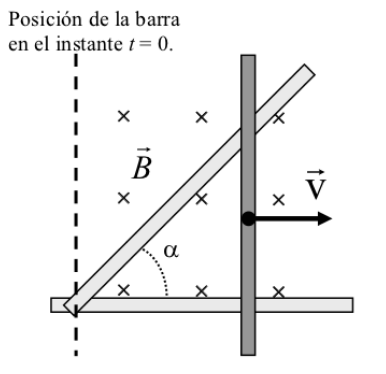
\includegraphics[scale=.5]{cir.png}
\end{minipage}
\qed
			
\end{enumerate}		
 
\end{document}

